\begin{proof}[Proof of Theorem~\ref{thm:antiLxP}] Let $A$ be a fixed point of $\varphi$. Assume first that $\ell(A)$ is even. Lemma~\ref{le:fixshape} gives that we must have edges $\big\{(x_0,y_0),(x_1,y_1),\ldots,(x_{2k},y_{2k})\big\}\subseteq G$
satisfying the conditions~\ref{lemma2.12_i} and~\ref{lemma2.12_ii}. If $k=0$, then $G=\{(1,m)\}$ and there is a unique fixed point $A=(\{1\},\{2,\ldots,m\})$. Now assume that $k>0$, in which case $y_{2k}=m$ and the edge $(x_{2k},y_{2k})$ is determined. With $i=k-1$ in condition~\ref{lemma2.12_i} of Lemma~\ref{le:fixshape} we have
\begin{equation}\label{eq:lastarcs}
G=
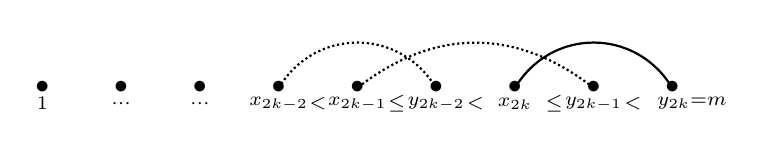
\begin{tikzpicture}[baseline=.2cm]
	\foreach \x in {1,3,5,7,9,11,13,15,17} 
		\node (\x) at (\x/2,0) [inner sep=-1pt] {$\bullet$};
	\node at (1/2,-.2) {$\scriptstyle 1$};
	\node at (2/2,-.2) {$\scriptstyle $};	
	\node at (3/2,-.2) {$\scriptstyle \cdots$};
	\node at (4/2,-.2) {$\scriptstyle $};	
	\node at (5/2,-.2) {$\scriptstyle \cdots$};
	\node at (6/2,-.2) {$\scriptstyle $};	
	\node at (7/2,-.2) {$\scriptstyle x_{2k-2}$};
	\node at (8/2,-.2) {$\scriptstyle <$};	
	\node at (9/2,-.2) {$\scriptstyle x_{2k-1}$};
	\node at (10/2,-.2) {$\scriptstyle \le$};	
	\node at (11/2,-.2) {$\scriptstyle y_{2k-2}$};
	\node at (12/2,-.2) {$\scriptstyle <$};	
	\node at (13/2,-.2) {$\scriptstyle x_{2k}$};
	\node at (14/2,-.2) {$\scriptstyle \le$};	
	\node at (15/2,-.2) {$\scriptstyle y_{2k-1}$};
	\node at (16/2,-.2) {$\scriptstyle <$};	
	\node at (17.5/2,-.2) {$\scriptstyle y_{2k}=m$};
	\draw [densely dotted,thick] (7) .. controls (8/2,.75) and (10/2,.75) .. (11); 
	\draw [densely dotted,thick] (9) .. controls (11/2,.75) and (13/2,.75) .. (15); 
	\draw [thick] (13) .. controls (14/2,.75) and (16/2,.75) .. (17); 
\end{tikzpicture} ,
 \end{equation}
 and condition~\ref{lemma2.12_ii} on the edges $(x_{2k-2},y_{2k-2})$, $(x_{2k-1},y_{2k-1})$ must also satisfy the condition~\ref{lemma2.12_ii} of Lemma~\ref{le:fixshape}. 
% Since $G$ has no nesting this
% implies that there is no edge $(x,y)\in G$ such that $y_{2k-2}<y<y_{2k-1}$. Hence the edges $(x_{2k-2},y_{2k-2})$ and $(x_{2k-1},y_{2k-1})$ are unique if they exist.
 Thus these edges $(x_{2k-1},y_{2k-1})$ and $(x_{2k-2},y_{2k-2})$ are uniquely determined and are such that they bound the vertex $x_{2k}$ on the right and on the left, respectively, i.e. $y_{2k-2}<x_{2k}\le y_{2k-1}$.
% If there is no such edges, then there is no fixed point with $\ell(A)$ even (\textbf{as this creates decomposibleness}). 
In this way, $\big\{(x_{2k-2},y_{2k-2}),(x_{2k-1},y_{2k-1}),(x_{2k},y_{2k})\big\}$ are uniquely determined.
 Now we can repeat the process with $i=k-2, k-3,\ldots,0$ in condition~\ref{lemma2.12_ii} 
% and (iii) 
 of Lemma~\ref{le:fixshape} to successively determine the edges $\big\{(x_0,y_0),(x_1,y_1),\ldots,(x_{2k},y_{2k})\big\}\subseteq G$, and the partition $A$ is given as in Lemma~\ref{le:fixshape}. 
 
 The case when the fixed point $A$ has odd length is very similar. The condition~\ref{lemma2.12_i} of Lemma~\ref{le:fixshape} gives $y_{2k+1}=m$ and hence determines the edge $(x_{2k+1},y_{2k+1})$ . 
Then condition~\ref{lemma2.12_ii} of Lemma~\ref{le:fixshape} with $i=k-1$ determines uniquely (if it exists) $(x_{2k},y_{2k})$ as the rightmost edge of $G$ such that $y_{2k}<y_{2k+1}$. Once $x_{2k}$ is determined
we continue the process as above with $i=k-2, k-3,\ldots,0$ to determine uniquely, if possible, all the other edges. Again, if at any time in the process we fail, then there is no fixed point with $\ell(A)$ odd. If we do not fail, there is a unique fixed point with $\ell(A)$ odd.

In conclusion, there are four possibilities. We could have no fixed point and in this case $c(G)=0$; we could have exactly one fixed point of odd length and $c(G)=-1$; we could have exactly one fixed point of even length and $c(G)=1$; or we have exactly two fixed points of different parity each and $c(G)=0$ in that case. In all cases Theorem~\ref{thm:antiLxP} follows. 
\end{proof}
